%----------------------------------------------------------------------------------------
%	PACKAGES AND OTHER DOCUMENT CONFIGURATIONS
%----------------------------------------------------------------------------------------

\documentclass{article}

\usepackage{fancyhdr} % Required for custom headers
\usepackage{lastpage} % Required to determine the last page for the footer
\usepackage{extramarks} % Required for headers and footers
\usepackage[usenames,dvipsnames]{color} % Required for custom colors
\usepackage{graphicx} % Required to insert images
\usepackage{listings} % Required for insertion of code
\usepackage{courier} % Required for the courier font
\usepackage{lipsum} % Used for inserting dummy 'Lorem ipsum' text into the template

% Margins
\topmargin=-0.45in
\evensidemargin=0in
\oddsidemargin=0in
\textwidth=6.5in
\textheight=9.0in
\headsep=0.25in

\linespread{1.1} % Line spacing

% Set up the header and footer
\pagestyle{fancy}
\chead{} % Top left header
\lhead{\hmwkClass\  \hmwkTitle} % Top center head
\rhead{} % Top right header
\lfoot{\lastxmark} % Bottom left footer
\cfoot{} % Bottom center footer
\rfoot{Page\ \thepage\ of\ \protect\pageref{LastPage}} % Bottom right footer
\renewcommand\headrulewidth{0.4pt} % Size of the header rule
\renewcommand\footrulewidth{0.4pt} % Size of the footer rule

\setlength\parindent{0pt} % Removes all indentation from paragraphs

%----------------------------------------------------------------------------------------
%	CODE INCLUSION CONFIGURATION
%----------------------------------------------------------------------------------------

% \definecolor{MyDarkGreen}{rgb}{0.0,0.4,0.0} % This is the color used for comments
\lstloadlanguages{C} % Load C syntax for listings, for a list of other languages supported see: ftp://ftp.tex.ac.uk/tex-archive/macros/latex/contrib/listings/listings.pdf
\lstset{language=C,frame=single,keywordstyle=[1]\color{Blue}\bf} % Use C in this example      



\newcommand{\csnippet}[2]{
\begin{itemize}
\item[]\lstinputlisting[caption=#2,label=#1]{#1.c}
\end{itemize}
}

%----------------------------------------------------------------------------------------
%	DOCUMENT STRUCTURE COMMANDS
%----------------------------------------------------------------------------------------

% Header and footer for when a page split occurs within a problem environment
\newcommand{\enterProblemHeader}[1]{
\nobreak\extramarks{#1}{#1 continued on next page\ldots}\nobreak
\nobreak\extramarks{#1 (continued)}{#1 continued on next page\ldots}\nobreak
}

% Header and footer for when a page split occurs between problem environments
\newcommand{\exitProblemHeader}[1]{
\nobreak\extramarks{#1 (continued)}{#1 continued on next page\ldots}\nobreak
\nobreak\extramarks{#1}{}\nobreak
}

\setcounter{secnumdepth}{0} % Removes default section numbers
\newcounter{homeworkProblemCounter} % Creates a counter to keep track of the number of problems

\newcommand{\homeworkProblemName}{}
\newenvironment{homeworkProblem}[1][Problem \arabic{homeworkProblemCounter}]{ % Makes a new environment called homeworkProblem which takes 1 argument (custom name) but the default is "Problem #"
\stepcounter{homeworkProblemCounter} % Increase counter for number of problems
\renewcommand{\homeworkProblemName}{#1} % Assign \homeworkProblemName the name of the problem
\section{\homeworkProblemName} % Make a section in the document with the custom problem count
\enterProblemHeader{\homeworkProblemName} % Header and footer within the environment
}{
\exitProblemHeader{\homeworkProblemName} % Header and footer after the environment
}

\newcommand{\problemAnswer}[1]{ % Defines the problem answer command with the content as the only argument
\noindent\framebox[\columnwidth][c]{\begin{minipage}{0.98\columnwidth}#1\end{minipage}} % Makes the box around the problem answer and puts the content inside
}

\newcommand{\homeworkSectionName}{}
\newenvironment{homeworkSection}[1]{ % New environment for sections within homework problems, takes 1 argument - the name of the section
\renewcommand{\homeworkSectionName}{#1} % Assign \homeworkSectionName to the name of the section from the environment argument
\subsection{\homeworkSectionName} % Make a subsection with the custom name of the subsection
\enterProblemHeader{\homeworkProblemName\ [\homeworkSectionName]} % Header and footer within the environment
}{
\enterProblemHeader{\homeworkProblemName} % Header and footer after the environment
}

%----------------------------------------------------------------------------------------
%	NAME AND CLASS SECTION
%----------------------------------------------------------------------------------------

\newcommand{\hmwkTitle}{Assignment\ \#1} % assignment title
\newcommand{\hmwkDueDate}{Monday,\ November\ 3,\ 2014} % due date
\newcommand{\hmwkClass}{Programming Concurrent Systems} % class
\newcommand{\hmwkClassTime}{} % lecture time
\newcommand{\hmwkClassInstructor}{} % lecturer
\newcommand{\hmwkAuthorName}{Alyssa - Ilias} %name

%----------------------------------------------------------------------------------------
%	TITLE PAGE
%----------------------------------------------------------------------------------------

\title{
\vspace{2in}
\textmd{\textbf{\hmwkClass:\ \hmwkTitle}}\\
\normalsize\vspace{0.1in}\small{Due\ on\ \hmwkDueDate}\\
\vspace{0.1in}\large{\textit{\hmwkClassInstructor\ \hmwkClassTime}}
\vspace{3in}
}

\author{\textbf{\hmwkAuthorName}}


%----------------------------------------------------------------------------------------

\begin{document}

\maketitle

%----------------------------------------------------------------------------------------
%	TABLE OF CONTENTS
%----------------------------------------------------------------------------------------

%\setcounter{tocdepth}{1} % Uncomment this line if you don't want subsections listed in the ToC

\newpage
\tableofcontents
\newpage

%----------------------------------------------------------------------------------------
%	Introduction
%----------------------------------------------------------------------------------------
\begin{homeworkProblem}[Introduction]
For this assignment we are asked to implement a simulation of heat dissipation on the surface of a cylinder. The implementation is sequential and will serve as a base to the following assignments where we will provide a parallelized solution.
\\\\
The surface is represented as a N x M matrix where each point is the temprature value. There is another same sized matrix where each point is the respective conductivity, where values are in the interval [0,1]. Depending on the conductivity of each point and its 8 surrounding neighbours, a new temprature is recomputed in an iterative manner. Specifically, the following formula describes the computations used for the simulation.
\\\\
\(t' = c_t*t + (1-c_t) * \frac{\sqrt{2}}{\sqrt{2}+1} * \frac{1}{4} * \sum_{i=1}^{4} a_i 
    + (1-c_t) * \frac{1}{\sqrt{2}+1} * \frac{1}{4} * \sum_{j=1}^{4} b_j \) , where 
\\\\
\(t'\) is the new temprature value \\
\(t\)  is the point's temprature value \\
\(c_t\) is the point's respective conductivity \\
\(a_i\) are the direct neighbour temprature values \\
\(b_j\) are the diagonal neighbour temprature values
\\\\
The M columns of the matrix represent the cyclic dimension of the cylinder so that tha first and last column are neighbours whereas the other dimension has fixed boundary on the first and last row. The repsective neighbours of the boundary have a fixed temprature of the initial temprature value.
\end{homeworkProblem}
%----------------------------------------------------------------------------------------
%	Solution Description
%----------------------------------------------------------------------------------------

% To have just one problem per page, simply put a \clearpage after each problem

\begin{homeworkProblem}[Solution Description]
In our solution we use two matrices. \textbf{t\_prev} and \textbf{t\_next}. The matrix \textbf{t\_prev} first contains the initial temprature values. Then in an iterative process we compute for every point the new value as depicted by Listing 1 and store in \textbf{t\_next}. When all points have been recomputed, we perform a swap on the two matrices. The iterative process ends when the maximum temprature difference is less than a user provided threshold, or the number of iterations have reached a user provided number.
\csnippet{main_calculation}{Snippet of the main calculation}
During the iterations we gather information on the heat dissipation process. This information is computed either every iteration or periodically depending on user input. We call this a reduction step. In the reduction step between other information we calculate the maximum temprature difference. It is important that we do a reduction step in order to effectively stop iterating in the case the difference is less than the threshold, but the reduction step also causes unnecessary overhead.
\\\\
Our first approach: \\
To deal with the boundary issue we do an explicit check whether we are on the first or last row and fetch the initial values directly from the input.\\
Similarly for the wraparound of the cyclic dimension we do an explicit check whether we are on the first or last column and fetch the opposite's value.
\\\\
After the optimization: \\
%@Alyssa append here
\end{homeworkProblem}

%----------------------------------------------------------------------------------------
%	Evaluation
%----------------------------------------------------------------------------------------

\begin{homeworkProblem}[Evaluation]
%\lipsum[2]
For the evaluation of our code we run a set of experiments. Following are the outcome observations:
\\\\
From the following graph we can see that if we do the reduction step on every iteration the impact is performance drawback. But we see that if we report periodically even often the overhead is little and the convergence is computed as well.
\\\\
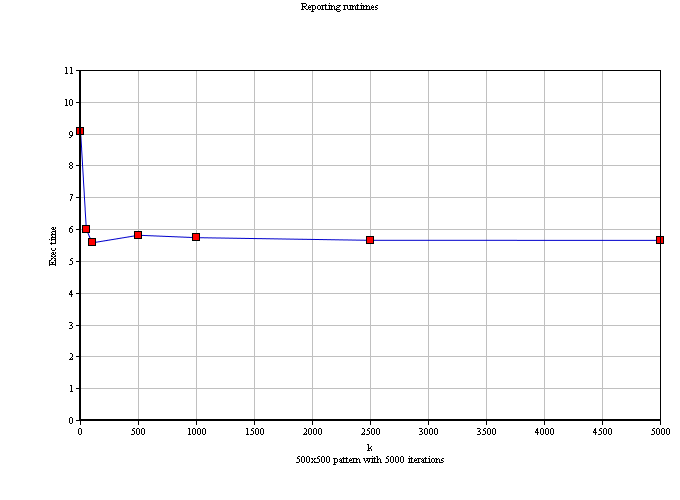
\includegraphics[width=0.75\columnwidth]{kshow.png}
%wrap with frame
%\problemAnswer{
%\begin{center}
%\includegraphics[width=0.75\columnwidth]{example_figure} % Example image
%\end{center}

%\lipsum[3-5]
%}
\end{homeworkProblem}

%----------------------------------------------------------------------------------------

\end{document}